% Created 2024-02-27 Tue 15:22
% Intended LaTeX compiler: pdflatex
\documentclass[presentation]{beamer}
\usepackage[utf8]{inputenc}
\usepackage[T1]{fontenc}
\usepackage{graphicx}
\usepackage{longtable}
\usepackage{wrapfig}
\usepackage{rotating}
\usepackage[normalem]{ulem}
\usepackage{amsmath}
\usepackage{amssymb}
\usepackage{capt-of}
\usepackage{hyperref}
\mode<beamer>{\usetheme{Madrid}}
\definecolor{SUred}{rgb}{0.59375, 0, 0.17969} % SU red (primary)
\definecolor{SUblue}{rgb}{0, 0.17578, 0.38281} % SU blue (secondary)
\setbeamercolor{palette primary}{bg=SUred,fg=white}
\setbeamercolor{palette secondary}{bg=SUblue,fg=white}
\setbeamercolor{palette tertiary}{bg=SUblue,fg=white}
\setbeamercolor{palette quaternary}{bg=SUblue,fg=white}
\setbeamercolor{structure}{fg=SUblue} % itemize, enumerate, etc
\setbeamercolor{section in toc}{fg=SUblue} % TOC sections
% Override palette coloring with secondary
\setbeamercolor{subsection in head/foot}{bg=SUblue,fg=white}
\setbeamercolor{date in head/foot}{bg=SUblue,fg=white}
\institute[SU]{Shenandoah University}
\titlegraphic{
\includegraphics[width=0.5\textwidth]{\string~/Documents/suLogo/suLogo.pdf}}
\usetheme{default}
\author{Chase Mathison\thanks{cmathiso@su.edu}}
\date{29 February 2024}
\title{Partial Fractions}
\hypersetup{
 pdfauthor={Chase Mathison},
 pdftitle={Partial Fractions},
 pdfkeywords={},
 pdfsubject={},
 pdfcreator={Emacs 29.1 (Org mode 9.6.7)}, 
 pdflang={English}}
\begin{document}

\maketitle

\section{Announcements}
\label{sec:orgb93f4ca}
\begin{frame}[label={sec:org673b113}]{Announcements}
\begin{enumerate}
\item Homework in MyOpenMath.
\item Office hours every weekday, 10am - 11am.
\item Trig Substitution quiz in Canvas, due Friday.
\end{enumerate}
\end{frame}

\section{Lecture}
\label{sec:orgaae9af0}
\begin{frame}[label={sec:org7a28c04}]{Partial Fractions}
Today's goal is to learn how to integrate functions such as
\[
\int\limits_{}^{} \frac{1}{x^2 \left( 1+x^2 \right)}\,dx \]
or
\[
\int\limits_{}^{} \frac{3x}{x^2-x}\,dx \]
in a way that is (arguably) easier than trigonometric substitution.

Trig substitution is still useful and necessary for integrals
involving \(\sqrt{a^2-x^2}\) and \(\sqrt{x^2-a^2}\) and
\(\sqrt{x^2+a^2}\), but when there's no square root in the
denominator, what we learn today will be an easier (and actually more
useful) method.
\end{frame}

\begin{frame}[label={sec:org5fb5a8c}]{Motivation}
The main motivation behind what we do today is the following:
Let's say we want to evaluate the integral
\[
\int\limits_{}^{} \frac{1}{x^2-2x}\,dx, \]
and you forgot for a moment (or don't want to do) trig substitution.

Well, then doing this integral is kind of hard.  But what if I told
you that
\[
\frac{1}{x^2-2x} = \frac{-1}{2x} + \frac{1}{2 \left( x-2 \right)}? \]
\end{frame}

\begin{frame}[label={sec:org999ce09}]{Motivation}
Then, we could find:
\[
\int\limits_{}^{} \frac{1}{x^2-2x}\,dx = \int \left( \frac{-1}{2x}
+\frac{1}{2 \left( x-2 \right)}\right)\,dx \]
And these integrals are much easier to handle!  We arrive at the
answer
\[
\int \frac{1}{x^2-2x}\,dx = \hspace{3in} \]
\end{frame}

\begin{frame}[label={sec:org08de7f2}]{Partial fraction decomposition}
Today we're going to focus on how to break down rational functions
like
\[
\frac{1}{x^2-2x} \] into \[\frac{-1}{2x} + \frac{1}{2 \left( x-2
\right)}. \]
This process is called finding the \uline{\hspace*{2in}}.
Using this method, we're going to be able (in theory) to integrate
\emph{any} rational function known to humankind!
\end{frame}

\begin{frame}[label={sec:org3834c91}]{The setup}
In general, we're trying to find a partial fraction decomposition of a
rational function \[\frac{P(x)}{Q(x)} \] where \(P(x)\) and \(Q(x)\)
are polynomials and \(\text{deg} \left( P(x) \right) < \text{deg}
\left( Q(x) \right)\).

Why do I have that restriction on the degrees of \(P\) and \(Q\)?
\vspace{10in}
\end{frame}

\begin{frame}[label={sec:org069df80}]{Example}
Use polynomial long division to simplify
\[
\frac{x^2-3x+1}{x-1}. \]

\vspace{10in}
\end{frame}
\begin{frame}[label={sec:orgd01a4fe}]{Partial fraction decomposition}
So, now that we know that we should only focus on rational functions
\(P \left( x \right)/Q \left( x \right)\) with the degree of \(P
\left( x \right)\) less than the degree of \(Q \left( x \right)\),
the most important thing we need to do is factor \(Q \left( x \right)\) correctly.

Depending on how \(Q \left( x \right)\) factors, there are a couple
of different paths we may take as far as setting up the partial
fraction decomposition.

Let's look at the easiest case that might occur: when \(Q (x)\) is a
product of \uline{\hspace*{1in}}, none of which repeat.
\end{frame}

\begin{frame}[label={sec:orgeb99cc5}]{Non repeating linear factors}
Let's say \(Q(x) = \left( a_1x + b_1 \right) \left( a_2x + b_2 \right)
\cdots \left( a_nx+b_n \right)\).  Then, we can write
\[
\frac{P(x)}{Q(x)} = \frac{P(x)}{\left( a_1x + b_1 \right) \left( a_2x + b_2 \right)
\cdots \left( a_nx+b_n \right)}. \]
The \alert{KEY STEP} to partial fractions is then writing this as:
\[
 \frac{P(x)}{\left( a_1x + b_1 \right) \left( a_2x + b_2 \right)
\cdots \left( a_nx+b_n \right)} = \hspace{3in}\]
(Don't let the \(n\) scare you\ldots{} most of the time \(Q (x)\) will
only have 2 or 3 factors in this class).
\end{frame}

\begin{frame}[label={sec:org4168913}]{Non repeating linear factors}
Let's pause and look at an example before moving on.

Find a partial fraction decomposition for the rational function
\[
\frac{2x-3}{x^2 - 4x - 5}. \]
\vspace{10in}
\end{frame}

\begin{frame}[label={sec:orgd591597}]{Non repeating linear factors}
\end{frame}

\begin{frame}[label={sec:org2147e9c}]{Application}
Find
\[\int\limits_{}^{} \frac{2x-3}{x^2-4x-5}\,dx. \]
\vspace{10in}
\end{frame}

\begin{frame}[label={sec:orgba4fffe}]{Equating coefficients and strategic substitution}
The last example illustrated the two main ways of find the constants
in the partial fraction decomposition \(A_1,A_2,\ldots,A_n:\) Equating
coefficients and strategic substitution.

Both methods will always work, but in the case of non repeating linear
factors of \(Q(x)\), strategic substitution is most of the time more
efficient.

We'll see later though, that sometimes equating coefficients is more
efficient.
\end{frame}

\begin{frame}[label={sec:org276abaa}]{Repeating linear factors}
Let's take another break for a second.

How would you calculate
\[
\frac{1}{x-1} + \frac{1}{(x-1)^2} + \frac{1}{x}?\]
You would get a common denominator of \(x(x-1)^2\) and add up to get 
\[
\hspace{1in}\]
\end{frame}

\begin{frame}[label={sec:org219af7f}]{Repeating linear factors}
From this we can see that when we're trying to find the partial
fraction decomposition of \[ \frac{2x^2-2x+1}{x(x-1)^2} \] that it's
not sufficient to only take it of the form
\[
\frac{A_1}{x-1} + \frac{A_2}{x} \text{ or } \frac{A_1}{(x-1)^2} +
\frac{A_2}{x} \]
but instead, we need to take the decomposition of the form
\[
\hspace{1in} \]
This illustrates what we need to do in general when \(Q(x)\) has
repeated linear factors
\end{frame}

\begin{frame}[label={sec:org7c5f300}]{Repeated linear factors}
\begin{block}{Rule: Linear factors}
If \(Q(x)\) has a factor of the form \((ax + b)^n\) where \(n\) is
a positive integer \(\ge 1\), then the partial fraction decomposition
of \(P(x)/Q(x)\) should contain
\[
\hspace{1in} \]
\phantom{butts}
\end{block}

You can still use the techniques of equating coefficients or strategic
substitution to solve for the constants in the partial fraction
decomposition.
\end{frame}

\begin{frame}[label={sec:org9edd409}]{Example}
Find the partial fraction decomposition of the rational function
\[
\frac{3x^2-3x-2}{\left( x^2-1 \right)\left( x-1 \right)^2}. \]
\vspace{10in}
\end{frame}

\begin{frame}[label={sec:orga30cc60}]{Example}
\end{frame}

\begin{frame}[label={sec:org4795f08}]{Example}
Find
\[
\int\limits_{}^{}\frac{3x^2-3x-2}{\left( x^2-1 \right)\left( x-1
\right)^2}\,dx. \]
\vspace{10in}
\end{frame}

\begin{frame}[label={sec:org379420a}]{Nonrepeating quadratic factors}
Sometimes when we're factoring \(Q(x)\), we might end up with
something that looks like
\[
Q(x) = \left( 2x+3 \right) \left( x^2 + 4 \right). \]
The issue here is that \(x^2+4\) can't be \uline{\hspace*{1in}} anymore using real
numbers no matter how hard we try.  It's not just a repeated linear
factor either: this is a totally new case for us.  
So, we need to figure out what to do when we have a factorization like
this. Fortunately, not much changes. 

For this specific example, we would have
\[
\frac{P(x)}{\left( 2x+3 \right)\left( x^2+4 \right)} =
\hspace{3in} \]
and we would again solve for \(A_1,A_2\) and now \(B_2\) using the
same methods as before.
\end{frame}

\begin{frame}[label={sec:org5cccfae}]{Example}
Find the partial fraction decomposition of the function
\[
\frac{1}{\left( 2x+3 \right)(x^2+4)} \]
\vspace{10in}
\end{frame}

\begin{frame}[label={sec:orgf2a494e}]{Example}
Find
\[
\int \frac{1}{\left( 2x+3 \right)(x^2+4)}\,dx\]
\vspace{10in}
\end{frame}

\begin{frame}[label={sec:org2209180}]{Repeating quadratic factors}
I don't think what's coming next is much of a surprise\ldots{}
\begin{block}{Rule: Quadratic factors}
If \(Q(x)\) has a repeated quadratic factor \((ax^2+bx+c)^n\), then
the partial fraction decomposition of \(P(x)/Q(x)\) should contain
terms of the form
\[
\hspace{1in} \]
\phantom{butts}
\end{block}
\end{frame}

\begin{frame}[label={sec:org4824929}]{Example}
Find the partial fraction decomposition of
\[
\frac{4x^3+2x^2+4}{\left( 2x^2+x+1 \right)^2}. \]
\vspace{10in}
\end{frame}

\begin{frame}[label={sec:orge38d794}]{Example}
\end{frame}

\begin{frame}[label={sec:org4e75950}]{Example}
Find
\[
\int\limits_{}^{} \frac{4x^3+2x^2+4}{\left( 2x^2+x+1 \right)^2}\,dx. \]
\vspace{10in}
\end{frame}

\begin{frame}[label={sec:orgfd7b26e}]{Putting it all together}
Here's an outline of all things partial fractions:

\begin{center}
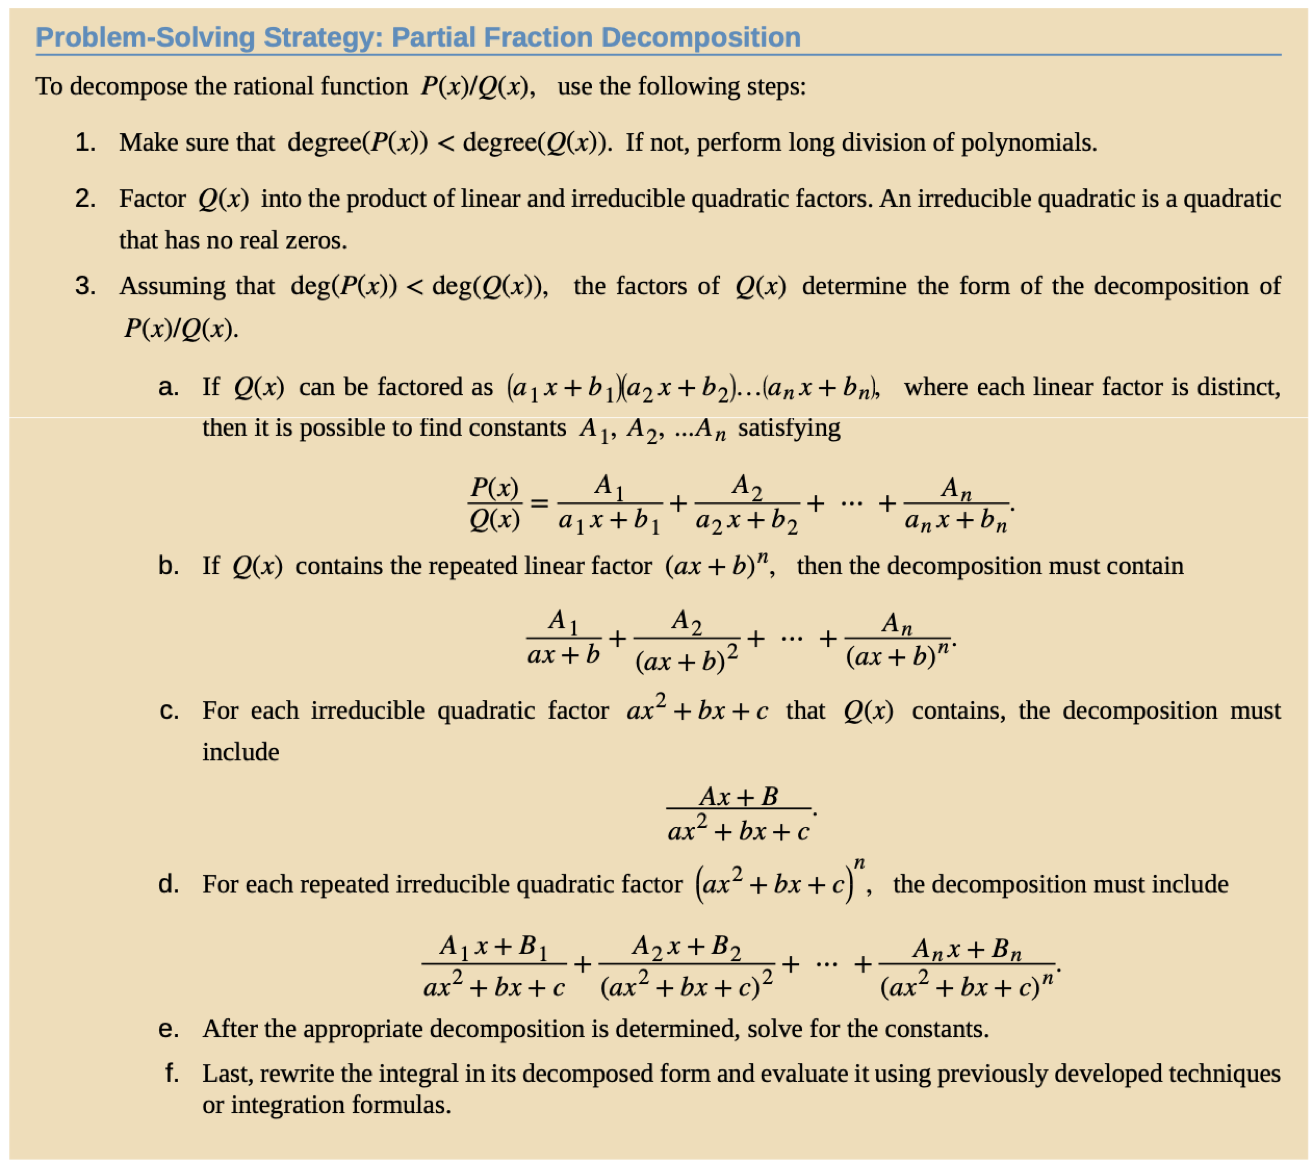
\includegraphics[width=0.7\textwidth]{../img/parfracF.png} \\
\end{center}
\end{frame}

\begin{frame}[label={sec:org2b54810}]{Examples}
Find
\[
\int\limits_{}^{} \frac{1}{x^3-8}\,dx \]
\vspace{10in}
\end{frame}

\begin{frame}[label={sec:org6060764}]{Examples}
\end{frame}

\begin{frame}[label={sec:orgaf80452}]{Examples}
Find the volume of the solid generated by rotating the region bounded
by the graph of
\[
f(x) = \frac{x^2}{\left( x^2+1 \right)^2} \]
and the \(x-\)axis between \(x=0\) and \(x=1\) about the \(y-\)axis.
\vspace{10in}
\end{frame}

\begin{frame}[label={sec:org8b4e8fa}]{Examples}
\end{frame}

\begin{frame}[label={sec:orgc414f70}]{Examples}
\end{frame}

\begin{frame}[label={sec:org194164d}]{Why only linear and quadratic factors}
At this point, you may ask:  What if \(Q (x)\) has factors that
aren't linear or quadratic?

That is a fantastic question, Chase.  It turns out though, that any
polynomial can be factored completely into (maybe repeated) linear and
quadratic factors.
Sometimes that factoring might be very very difficult to do, but it's
always technically possible.  So, we've actually studied all of the
cases we need to for partial fractions!  Time to celebrate!
\end{frame}
\end{document}